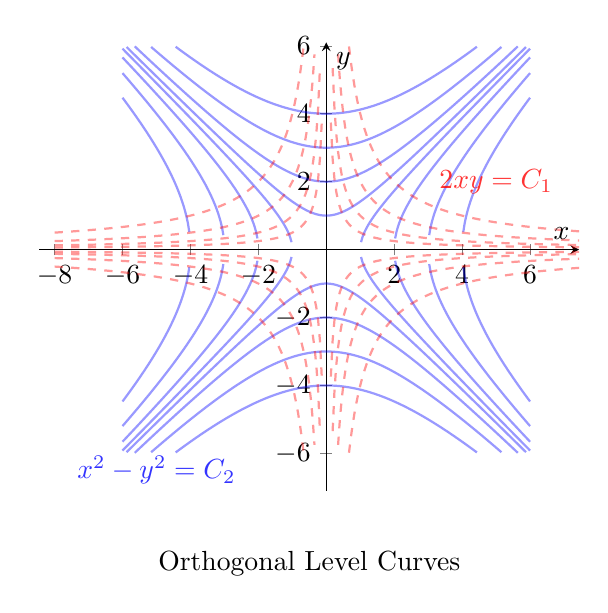
\begin{tikzpicture}
  \begin{axis}[
    axis equal,
    axis lines=middle,
    xmin=-6, xmax=5,
    ymin=-6, ymax=5,
    xlabel={$x$}, ylabel={$y$},
    samples=300,
    domain=-6:6,
    restrict y to domain=-6:6,
    enlargelimits=true,
    title={ Orthogonal Level Curves},
    title style={at={(0.5,-0.15)}, anchor=north},
  ]

  % Real part level curves: u(x,y) = x^2 - y^2 = c (solid blue)
  \foreach \c in {-16,-9,-4,-1,1,4,9,16} {
    \addplot [blue, thick, opacity=0.4, domain=-6:6]
      ({x}, {sqrt(x^2 - \c)});
    \addplot [blue, thick, opacity=0.4, domain=-6:6]
      ({x}, {-sqrt(x^2 - \c)});
  }

  % Imaginary part level curves: v(x,y) = 2xy = c (dashed red)
  \foreach \c in {-8,-4,-2,-1,1,2,4,8} {
    \addplot [red, thick, dashed, opacity=0.4, domain=-8:8, samples=300]
      ({x}, {\c/(2*x)});
  }
% $f(x, y) = (x^2 - y^2,\ 2xy)$:
  \node at (axis cs:5, 2.0) [red,  opacity=0.8] {$2xy=C_1$};
  \node at (axis cs:-5., -6.5) [blue, opacity=0.8] {$x^2 - y^2=C_2$};

  \end{axis}
\end{tikzpicture}